\section{Modelos de datos}\label{sec:modelo}
Los modelos de datos son una representación estructurada de la información
almacenada que se utiliza para almacenar, recuperar y manipular los datos de
forma eficiente. En este caso, se definirán los modelos de datos que se
ingestarán en el sistema, así como las relaciones entre ellos y las
características de cada uno.

Cada uno de los modelos de datos se corresponde con una fuente de datos
diferente, y se utilizarán para analizar y visualizar la información de manera
eficiente.

\emph{NOTA: por confidencialidad, no se mostrarán los modelos de datos internos
de Okticket (hojas de gastos, reportes, usuarios, compañías, etc.).}


\newpage{}
\subsection{Logs de balanceadores (AWS)}
Los registros de los balanceadores de carga de AWS contienen información
sobre las solicitudes que se realizan a los servicios de la aplicación. En la
figura \ref{fig:logs_elb} se muestra el modelo de datos de estos registros.

Estos registros contienen información muy valiosa sobre el tráfico de la
empresa, y permiten identificar métricas así como problemas de infraestructura
de manera rápida y eficiente.

\begin{figure}[H]
	\centering
	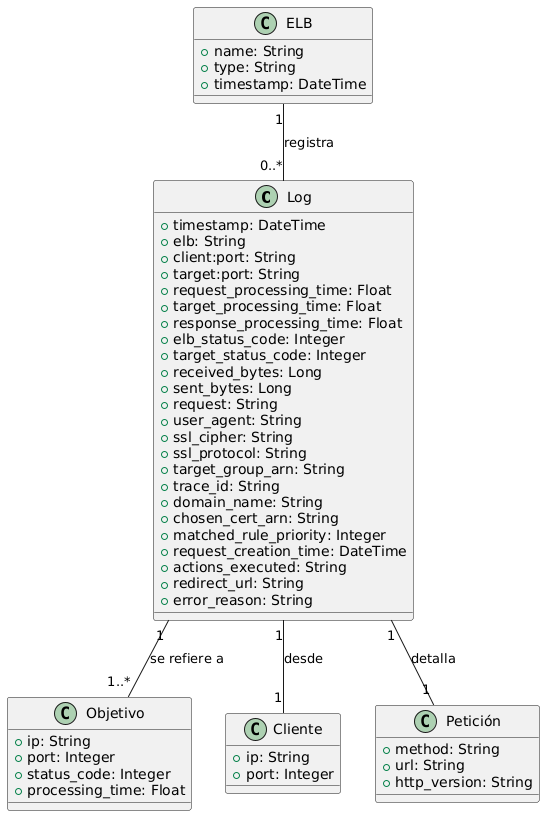
\includegraphics[width=0.65\textwidth]{uml/logs_elb.png}
	\caption{Modelo de datos de los logs de un balanceador de carga de AWS}
	\label{fig:logs_elb}
\end{figure}


\newpage{}
\subsection{Logs de bases de datos SQL}
Los registros de las bases de datos SQL contienen información sobre las
consultas que se realizan a la base de datos, así como errores y otros eventos
importantes. En la figura \ref{fig:logs_sql} se muestra el modelo de datos de
estos registros.

\begin{figure}[H]
	\centering
	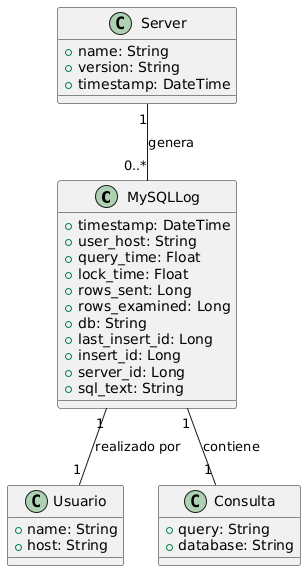
\includegraphics[width=0.4\textwidth]{uml/logs_sql.png}
	\caption{Modelo de datos de los logs de una base de datos SQL}
	\label{fig:logs_sql}
\end{figure}


\newpage{}
\subsection{Logs de bases de datos MongoDB}
Los registros de las bases de datos MongoDB contienen información sobre las
operaciones que se realizan en la base de datos, así como errores y otros
eventos importantes. En la figura \ref{fig:logs_mongo} se muestra el modelo de
datos de estos registros.

\begin{figure}[H]
	\centering
	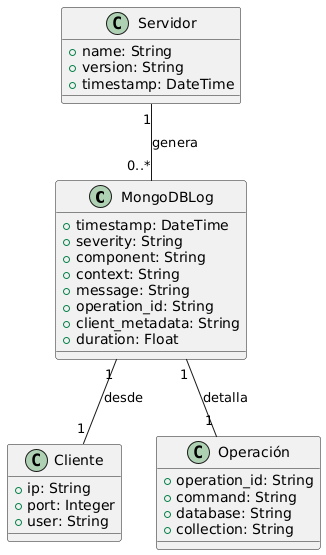
\includegraphics[width=0.4\textwidth]{uml/logs_mongo.png}
	\caption{Modelo de datos de los logs de una base de datos MongoDB}
	\label{fig:logs_mongo}
\end{figure}


\newpage{}
\subsection{Logs de Laravel (API)}
Los logs de Laravel contienen, entre otras cosas, información sobre los
errores y excepciones que se producen en el \textit{backend} de la
aplicación.

Para un análisis completo del estado de la aplicación (en el caso de
Okticket), se deben analizar los logs de todos los despliegues de la
API, ya que cada uno de ellos puede contener información relevante.

\begin{figure}[H]
	\centering
	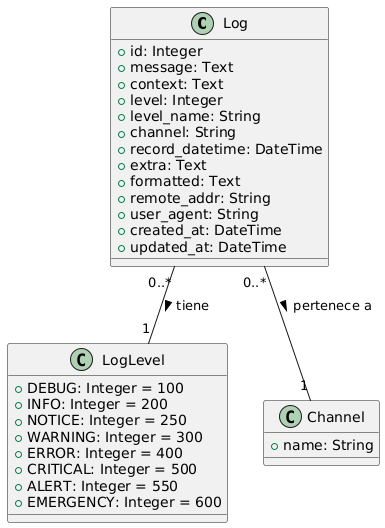
\includegraphics[width=0.5\textwidth]{uml/logs_laravel.png}
	\caption{Modelo de datos de los logs de una aplicación Laravel}
	\label{fig:logs_laravel}
\end{figure}
